\documentclass{article}
\usepackage[utf8]{inputenc}
\usepackage{subfig}
\usepackage{amsmath}

\usepackage{graphicx}
\usepackage[legalpaper, portrait, margin=0.5cm]{geometry}

\thispagestyle{empty}
\renewcommand{\thesubfigure}{\roman{subfigure}}

\begin{document}

\begin{figure}[h]
        \centering
        \subfloat[spectrum]{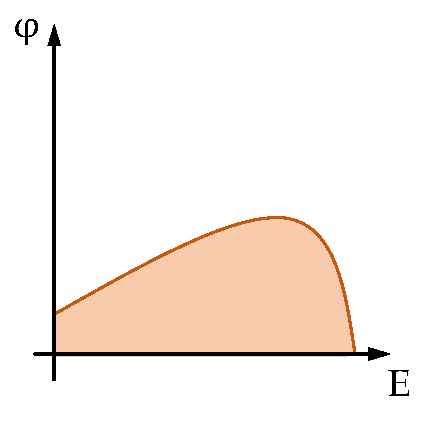
\includegraphics[height=3.1cm]{figures/ch02/bm_spectrum.pdf}}
        \subfloat[emission profile]{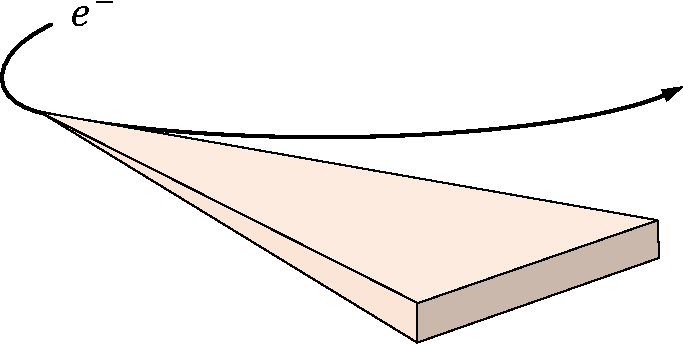
\includegraphics[width=7cm]{figures/ch02/bm.pdf}}
        \\ \setcounter{subfigure}{0}% Reset subfigure counter

        \caption*{(a) bending magnet radiation}
        
        \subfloat[spectrum]{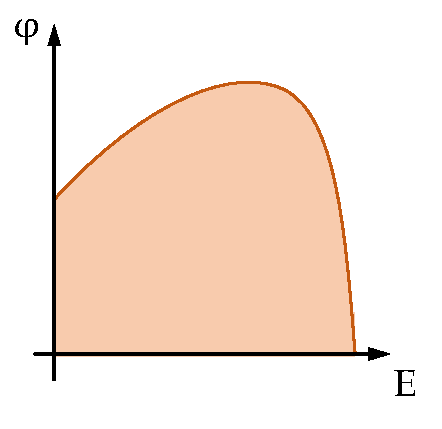
\includegraphics[height=3.1cm]{figures/ch02/w_spectrum.pdf}}
        \subfloat[emission profile]{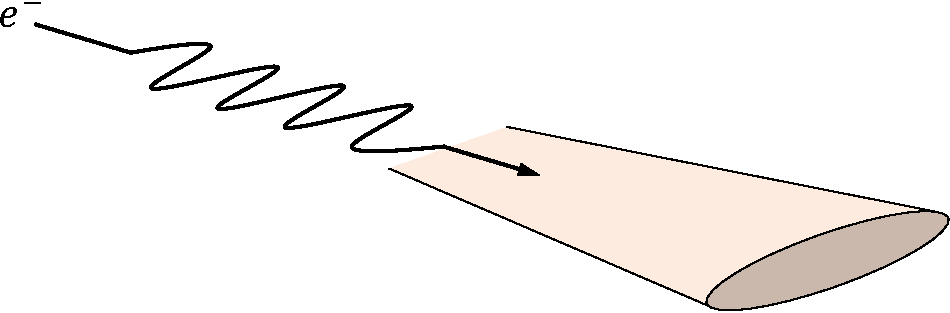
\includegraphics[width=7cm]{figures/ch02/w.pdf}}
        \\ \setcounter{subfigure}{0}% Reset subfigure counter

        \caption*{(b) wiggler radiation}
        
        \subfloat[spectrum]{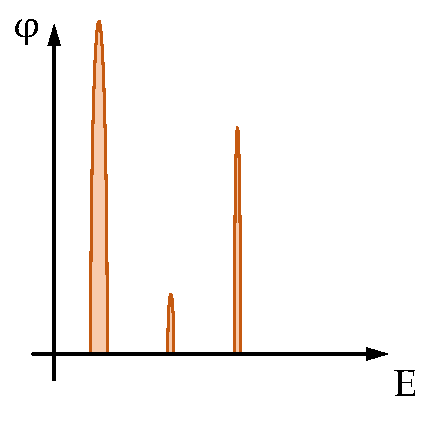
\includegraphics[height=3.1cm]{figures/ch02/u_spectrum.pdf}}
        \subfloat[emission profile]{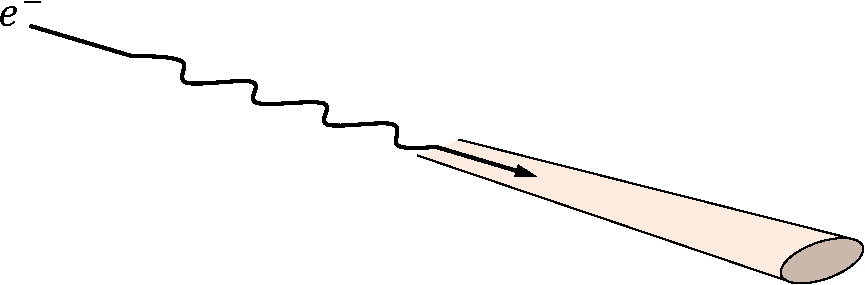
\includegraphics[width=7cm]{figures/ch02/u.pdf}}
        \\ \setcounter{subfigure}{0}% Reset subfigure counter

        \caption*{(c) undulator radiation}

        
\end{figure}


\end{document}